\section{Optimisasi CMA-ES}

\subsection{Gambaran Umum}

\textbf{Covariance Matrix Adaptation Evolution Strategy (CMA-ES)} adalah algoritma optimisasi numerik stokastik tanpa turunan yang kuat dengan karakteristik berikut:

\begin{itemize}
    \item Algoritma optimisasi numerik stokastik tanpa turunan yang kuat.
    \item \textbf{Tipe:} Algoritma Evolusioner (domain kontinu).
    \item \textbf{Kasus Penggunaan:} Fungsi objektif non-konveks, tidak terkondisi dengan baik, multimodal, atau berisik.
    \item \textbf{Relevansi dengan VQE:} Digunakan untuk mengoptimalkan parameter $\boldsymbol{\theta}$ dari sirkuit variasional ketika gradien sulit dihitung atau berisik (misalnya, pada perangkat keras NISQ).
\end{itemize}

\subsection{Cara Kerja CMA-ES}

Algoritma mempertahankan distribusi Gaussian $\mathcal{N}(m, \sigma^2 C)$ dan memperbaruinya secara iteratif:

\begin{enumerate}
    \item \textbf{Pengambilan Sampel:} Menghasilkan populasi solusi kandidat baru (keturunan) dari distribusi saat ini.
    \item \textbf{Seleksi:} Mengevaluasi kebugaran (energi) dan memilih kandidat terbaik.
    \item \textbf{Adaptasi:} Memperbarui parameter distribusi:
        \begin{itemize}
            \item \textbf{Mean ($m$):} Bergerak menuju solusi yang lebih baik.
            \item \textbf{Ukuran Langkah ($\sigma$):} Mengontrol eksplorasi vs. eksploitasi.
            \item \textbf{Matriks Kovarian ($C$):} Mempelajari bentuk lanskap (korelasi antar variabel) untuk memandu pencarian.
        \end{itemize}
\end{enumerate}

\subsection{Ilustrasi Proses CMA-ES}

Proses optimisasi CMA-ES dapat divisualisasikan melalui beberapa langkah:

\begin{enumerate}
    \item \textbf{Inisialisasi:} Pencarian dimulai dengan mean awal dan distribusi yang luas.
    \begin{center}
        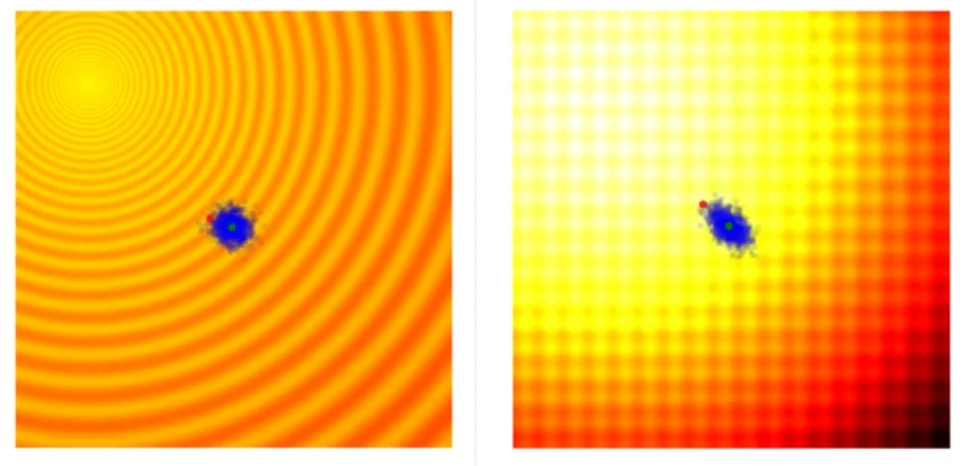
\includegraphics[width=0.7\textwidth]{Step1.png}
    \end{center}
    \item \textbf{Pengambilan Sampel \& Seleksi:} Kandidat diambil sampelnya; yang terbaik (biru) dipilih untuk memandu pembaruan.
    \begin{center}
        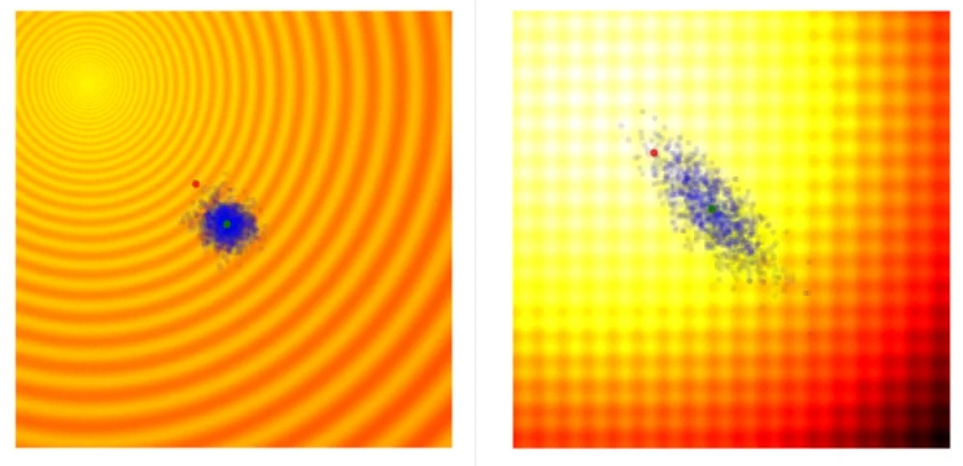
\includegraphics[width=0.7\textwidth]{Step2.png}
    \end{center}
    \item \textbf{Adaptasi:} Distribusi bergeser dan membentuk ulang (pembaruan kovarian) menuju lembah.
    \begin{center}
        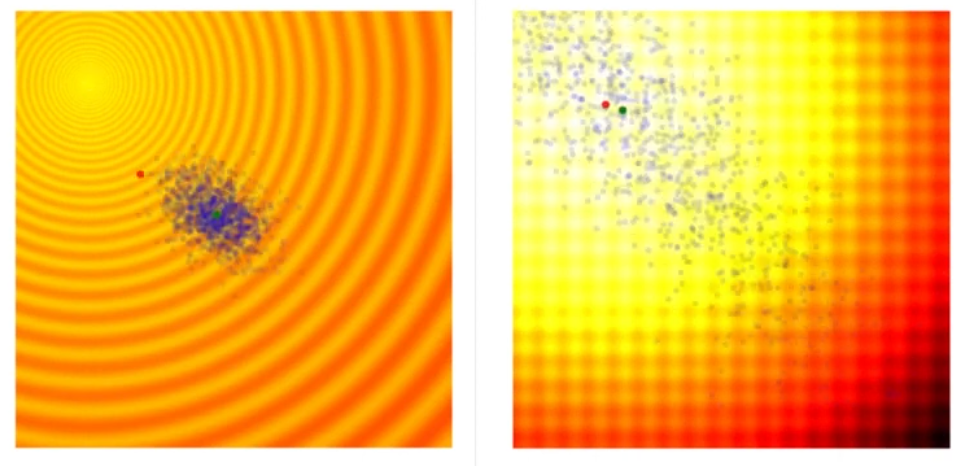
\includegraphics[width=0.7\textwidth]{Step3.png}
    \end{center}
    \item \textbf{Eksplorasi:} Algoritma mengeksplorasi lanskap, memanjang sepanjang arah optimal.
    \begin{center}
        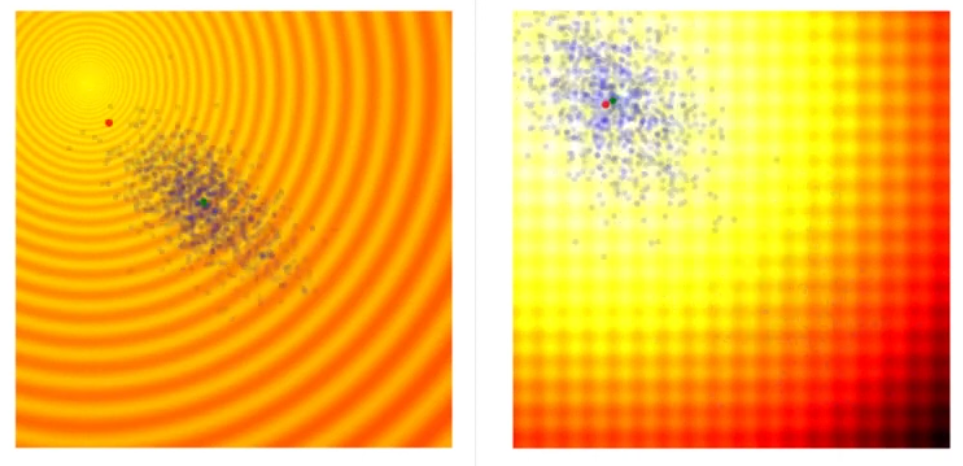
\includegraphics[width=0.7\textwidth]{Step4.png}
    \end{center}
    \item \textbf{Konvergensi Dimulai:} Ukuran langkah menurun saat populasi berpusat pada minimum.
    \begin{center}
        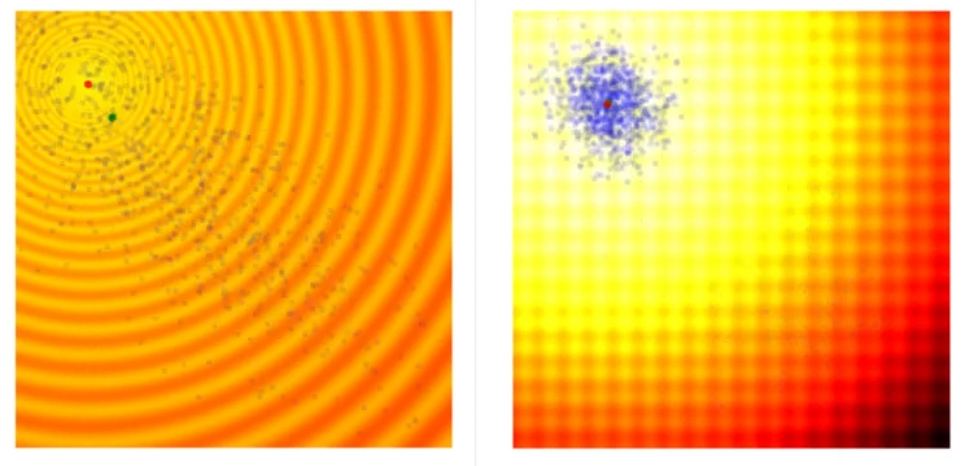
\includegraphics[width=0.7\textwidth]{Step5.png}
    \end{center}
    \item \textbf{Penyetelan Halus:} Lokalisasi presisi dari optimum.
    \begin{center}
        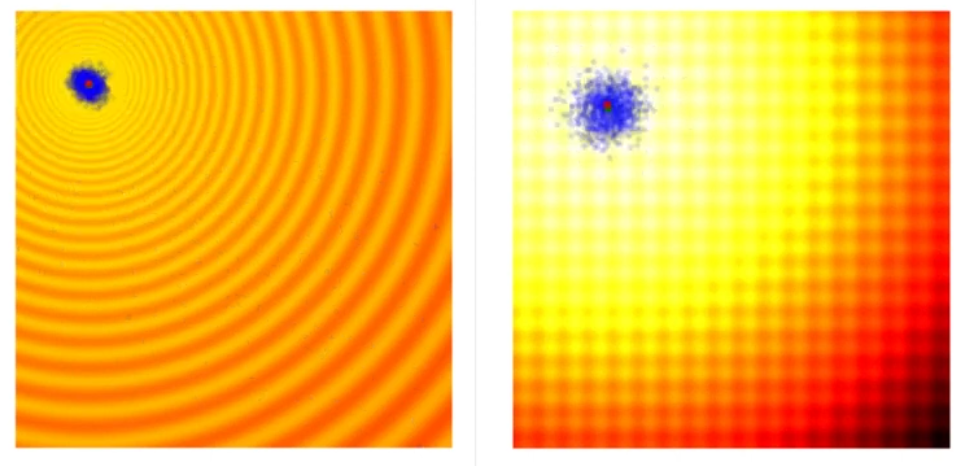
\includegraphics[width=0.7\textwidth]{Step6.png}
    \end{center}
    \item \textbf{Optimisasi Selesai:} Distribusi konvergen ke minimum global.
    \begin{center}
        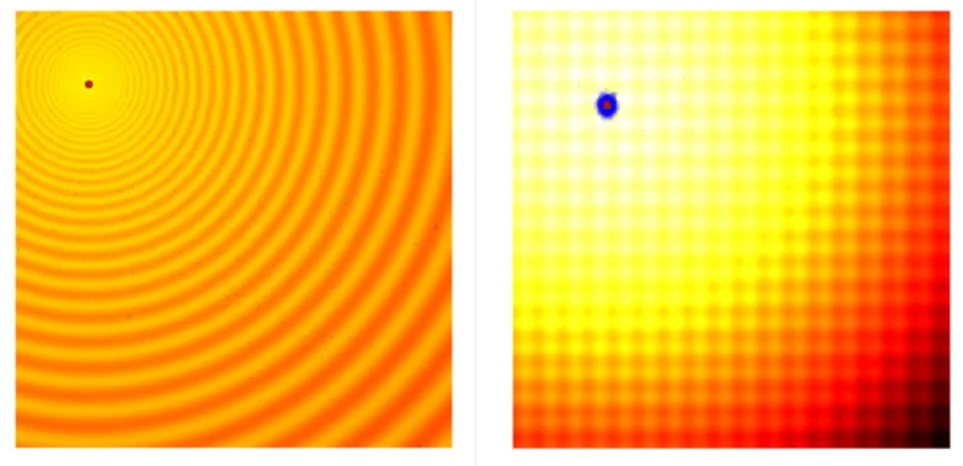
\includegraphics[width=0.7\textwidth]{Step7.png}
    \end{center}
\end{enumerate}
